\documentclass{article}
\usepackage{amsmath}
\usepackage{amssymb}
\usepackage{graphicx}
\usepackage{hyperref}
\usepackage[version=4]{mhchem}

\title{Problem 8}
\date{}

\begin{document}
\maketitle

\section*{Problem}
(AMC) Triangle \(A B C\) and point \(P\) in the same plane are given. Point \(P\) is equidistant from \(A\) and \(B\), angle \(A P B\) is twice angle \(A C B\), and \(A C\) intersects \(B P\) at point \(D\). If \(P B=3\) and \(P D=2\), then \(A D \cdot C D=\)\\
(A) 5\\
(B) 6\\
(C) 7\\
(D) 8\\
(E) 9\\
\centering
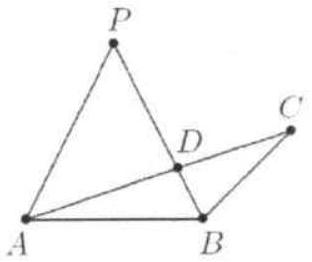
\includegraphics[width=\textwidth]{images/207(2).jpg}

\section*{Solution}
(A).\\
Method 1:\\
Construct a circle with center \(P\) and radius \(P A\). Point \(C\) then lies on the circle, since the angle \(A C B\) is half angle \(A P B\).

Extend \(B P\) through \(P\) to get diameter \(B E\). Since \(A, B, C\), and \(E\) are concyclic, using the Power of a Point formula, we have:\\
\centering
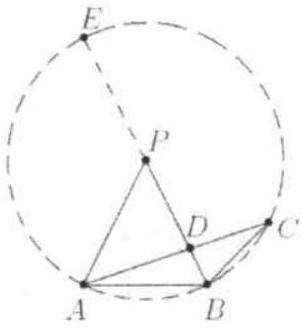
\includegraphics[width=\textwidth]{images/211(1).jpg}\\
\(A D \cdot C D=E D \cdot B D\)\\
\(=(P E+P D)(P B-P D)=(3+2)(3-2)=5\).\\
Method 2:\\
Extend \(B P\) to \(E\) such that \(P E=P B\). Since \(P A=P B=P E\), points \(A, B\), and \(E\) are concyclic. Construct this semicircle with center \(P\) as shown in the figure to the right.\\
So we have \(\angle A E B=\frac{1}{2} \angle A P B=\angle A C B\). We also know that\\
\centering

\includegraphics[width=\textwidth]{images/211.jpg}


\(\angle A D E=\angle B D C\) (vertical angles). Therefore \(\triangle A E D \sim \triangle D C B\).\\
\(\frac{A D}{B D}=\frac{E D}{D C} \Rightarrow A D \cdot C D=E D \cdot B D=(P E+P D)(P B-P D)\)\\
\(=(3+2)(3-2)=5\).

\end{document}
